\section{Use Hierarchy Between Modules}\label{SecUse}

\citet{Parnas1978} said of two programs, A and B, that A {\em uses} B if the
correct execution of B might be necessary for A to complete the task as
specified. That is, A {\em uses} B if there exist situations in which the
correct functioning of A depends upon the availability of a correct
implementation of B.

The \textit{uses} hierarchy between modules (Figure~\ref{FigUH}) shows that the
graph is a directed acyclic graph (DAG). Each level of the hierarchy offers a
testable and usable subset of the system. Modules in the higher level of the
hierarchy are simpler because they use modules from the lower levels.

\vspace*{\fill}
\begin{figure}[!tbh]
    \centering
    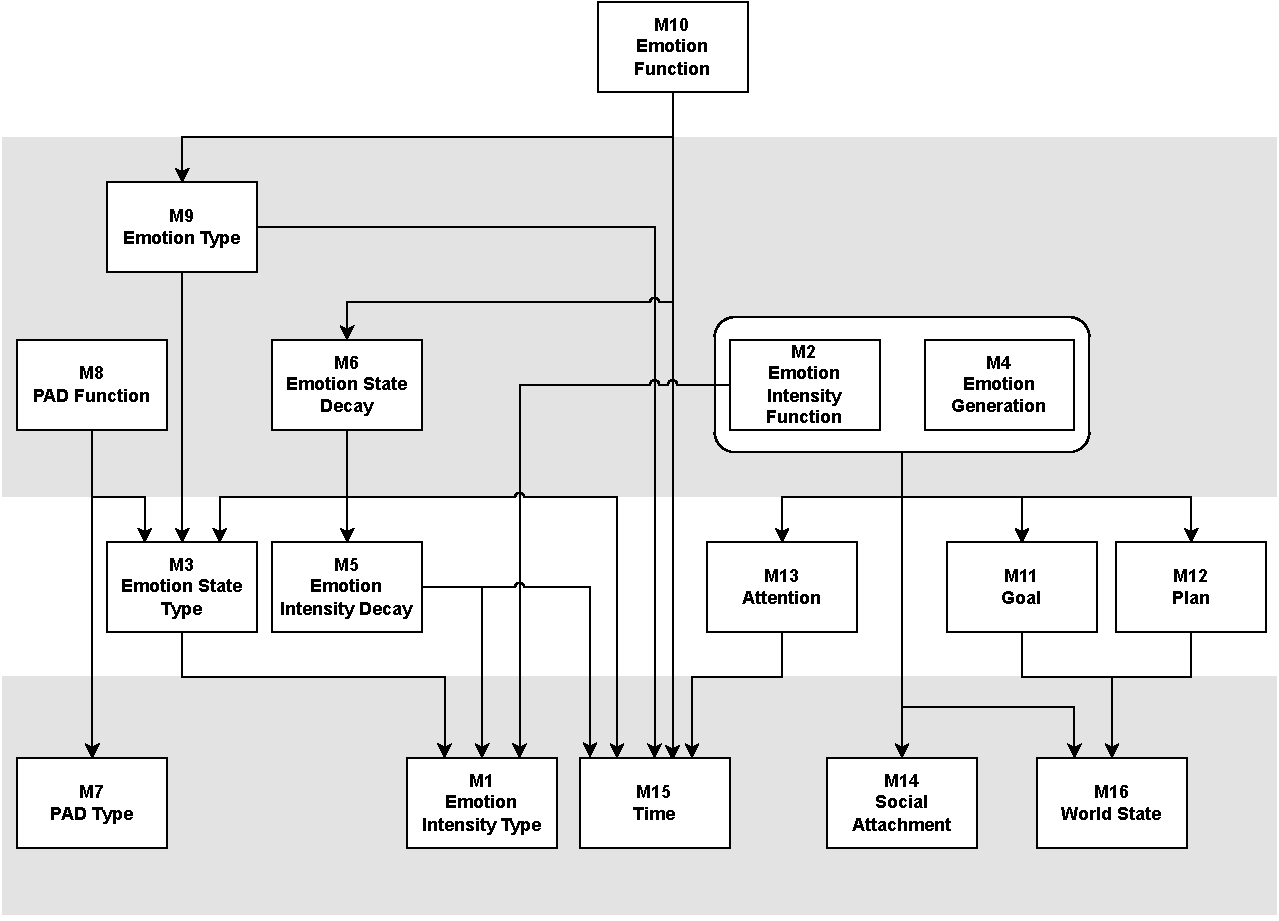
\includegraphics[width=\linewidth]{figures/usesHierarchy.pdf}
    \caption{Use hierarchy among modules}
    \label{FigUH}
\end{figure}
\vspace*{\fill}